% Created 2015-01-26 Mon 00:50
\documentclass[11pt]{book}
\usepackage{graphicx}
\usepackage{xcolor}
\usepackage{xeCJK}
\setCJKmainfont{SimSun}
\usepackage{longtable}
\usepackage{float}
\usepackage{textcomp}
\usepackage{geometry}
\geometry{left=0cm,right=0cm,top=0cm,bottom=0cm}
\usepackage{multirow}
\usepackage{multicol}
\usepackage{listings}
\usepackage{algorithm}
\usepackage{algorithmic}
\usepackage{latexsym}
\usepackage{natbib}
\usepackage{fancyhdr}
\usepackage[xetex,colorlinks=true,CJKbookmarks=true,linkcolor=blue,urlcolor=blue,menucolor=blue]{hyperref}


\lstset{language=Java,numbers=left,numberstyle=\tiny,basicstyle=\ttfamily\small,tabsize=4,frame=none,escapeinside=``,extendedchars=false,keywordstyle=\color{blue!70},commentstyle=\color{red!55!green!55!blue!55!},rulesepcolor=\color{red!20!green!20!blue!20!}}
\author{deepwaterooo}
\date{\today}
\title{LeetCode Summary}
\hypersetup{
  pdfkeywords={},
  pdfsubject={},
  pdfcreator={Emacs 24.3.1 (Org mode 8.2.7c)}}
\begin{document}

\maketitle
\tableofcontents


\chapter{线性表}
\label{sec-1}
\section{Array}
\label{sec-1-1}
\subsection{Two Sum}
\label{sec-1-1-1}
\subsection{Two Sum II - Input Array is Sorted}
\label{sec-1-1-2}
\subsection{Two Sum III - Data Structure Design}
\label{sec-1-1-3}

\subsection{Valid Palindrome}
\label{sec-1-1-4}
\section{单链表: Single Linked List}
\label{sec-1-2}

\chapter{字符串: String}
\label{sec-2}

\subsection{Implement strStr()}
\label{sec-2-0-1}
\subsection{Reverse Words in a String}
\label{sec-2-0-2}
\subsection{Reverse Words in a String II}
\label{sec-2-0-3}
\subsection{String to Integer (atoi)}
\label{sec-2-0-4}
\subsection{Valid Number}
\label{sec-2-0-5}
\subsection{Longest Substring Without Repeating Characters}
\label{sec-2-0-6}
\subsection{Longest Substring with At Most Two Distinct Characters}
\label{sec-2-0-7}
\subsection{Longest Palindromic Substring}
\label{sec-2-0-8}
\subsection{Missing Ranges}
\label{sec-2-0-9}
\subsection{One Edit Distance}
\label{sec-2-0-10}
\subsection{Read N Characters Given Read4}
\label{sec-2-0-11}
\subsection{Read N Characters Given Read4 II - Call multiple times}
\label{sec-2-0-12}
\chapter{Linked List}
\label{sec-3}

\section{Easier Maybe?}
\label{sec-3-1}
\subsection{Merge Two Sorted List}
\label{sec-3-1-1}
\subsection{Add Two Numbers}
\label{sec-3-1-2}
\subsection{Swap Nodes in Pairs}
\label{sec-3-1-3}
\subsection{Copy List With Random Pointers}
\label{sec-3-1-4}
\chapter{树: Binary Tree, Binary Search Tree}
\label{sec-4}
\section{二叉树的遍历}
\label{sec-4-1}
\subsection{}
\label{sec-4-1-1}
\section{二叉树的构建}
\label{sec-4-2}
\subsection{}
\label{sec-4-2-1}
\section{二叉树查找}
\label{sec-4-3}
\section{二叉树递归}
\label{sec-4-4}

\chapter{栈和队列}
\label{sec-5}
\section{栈}
\label{sec-5-1}
\subsection{Evaluate Reverse Polish Notation}
\label{sec-5-1-1}
\subsection{Valid Parentheses}
\label{sec-5-1-2}
\subsection{}
\label{sec-5-1-3}
\section{队列}
\label{sec-5-2}
\subsection{}
\label{sec-5-2-1}
\section{Heap: Merge k sorted List}
\label{sec-5-3}
Merge k sorted linked lists and return it as one sorted list. Analyze and describe its complexity.
\textbf{Tags}: Divide and Conquer, Linked List, Heap
\lstset{language=java,label= ,caption= ,numbers=none}
\begin{lstlisting}
public ListNode mergeTwoLists(ListNode l1, ListNode l2) {
    if (l1 == null) return l2;
    if (l2 == null) return l1;
    ListNode result;
    if (l1.val < l2.val) {
        result = l1;
        l1 = l1.next;
        result.next = null;
    } else {
        result = l2;
        l2 = l2.next;
        result.next = null;
    }
    ListNode curr = result;
    while (l1 != null && l2 != null) {
        if (l1.val < l2.val) {
            curr.next = l1;
            curr = curr.next;
            l1 = l1.next;
            curr.next = null;
        } else {
            curr.next = l2;
            curr = curr.next;
            l2 = l2.next;
            curr.next = null;
        }
    }
    if (l1 == null && l2 == null)
        return result;
    l1 = (l1 == null) ? l2 : l1;
    curr.next = l1;
    return result;
}

public ListNode mergeKLists(List<ListNode> lists) {
    if (lists.size() == 0) return null;
    if (lists.size() == 1) return lists.get(0);
    if (lists.size() == 2) return mergeTwoLists(lists.get(0), lists.get(1));
    return mergeTwoLists((mergeKLists(lists.subList(0, lists.size() / 2))),
                         (mergeKLists(lists.subList(lists.size() / 2, lists.size()))));
}
\end{lstlisting}

\chapter{Backtracing and Recursion}
\label{sec-6}
\section{排列: Permutation}
\label{sec-6-1}
\subsection{Permutation}
\label{sec-6-1-1}
Given a collection of numbers, return all possible permutations.

For example,
\lstset{language=java,label= ,caption= ,numbers=none}
\begin{lstlisting}
[1,2,3] have the following permutations:
[1,2,3], [1,3,2], [2,1,3], [2,3,1], [3,1,2], and [3,2,1].
\end{lstlisting}
\subsection{Permutation II}
\label{sec-6-1-2}
Given a collection of numbers that might contain duplicates, return all possible unique permutations.

For example,
\lstset{language=java,label= ,caption= ,numbers=none}
\begin{lstlisting}
[1,1,2] have the following unique permutations:
[1,1,2], [1,2,1], and [2,1,1].
\end{lstlisting}
\subsection{Permutation Sequence}
\label{sec-6-1-3}
The set [1,2,3,…,n] contains a total of n! unique permutations.

By listing and labeling all of the permutations in order, We get the following sequence (ie, for n = 3):
\lstset{language=java,label= ,caption= ,numbers=none}
\begin{lstlisting}
"123"
"132"
"213"
"231"
"312"
"321"
\end{lstlisting}
Given n and k, return the kth permutation sequence.

Note: Given n will be between 1 and 9 inclusive.
\section{组合:Combination}
\label{sec-6-2}
\subsection{Combinationas}
\label{sec-6-2-1}
Given two integers n and k, return all possible combinations of k numbers out of 1 \ldots{} n.

For example,

If n = 4 and k = 2, a solution is:
\lstset{language=java,label= ,caption= ,numbers=none}
\begin{lstlisting}
[
  [2,4],
  [3,4],
  [2,3],
  [1,2],
  [1,3],
  [1,4],
]
\end{lstlisting}
\subsection{Combination Sum}
\label{sec-6-2-2}
Given a set of candidate numbers (C) and a target number (T), find all unique combinations in C where the candidate numbers sums to T.

The same repeated number may be chosen from C unlimited number of times.

Note:
\begin{itemize}
\item All numbers (including target) will be positive integers.
\item Elements in a combination (a1, a2, … , ak) must be in non-descending order. (ie, a1 ≤ a2 ≤ … ≤ ak).
\item The solution set must not contain duplicate combinations.
\end{itemize}

For example, given candidate set 2,3,6,7 and target 7, 

A solution set is: 
\lstset{language=java,label= ,caption= ,numbers=none}
\begin{lstlisting}
[7] 
[2, 2, 3]
\end{lstlisting}
\subsection{Combination Sum II}
\label{sec-6-2-3}
Given a collection of candidate numbers (C) and a target number (T), find all unique combinations in C where the candidate numbers sums to T.

Each number in C may only be used once in the combination.

Note:
\begin{itemize}
\item All numbers (including target) will be positive integers.
\item Elements in a combination (a1, a2, … , ak) must be in non-descending order. (ie, a1 ≤ a2 ≤ … ≤ ak).
\item The solution set must not contain duplicate combinations.
\end{itemize}
For example, given candidate set 10,1,2,7,6,1,5 and target 8, 

A solution set is: 
\lstset{language=java,label= ,caption= ,numbers=none}
\begin{lstlisting}
[1, 7] 
[1, 2, 5] 
[2, 6] 
[1, 1, 6]
\end{lstlisting}
\section{Subsets}
\label{sec-6-3}
\subsection{Subsets: Bit Manipulation}
\label{sec-6-3-1}
Given a set of distinct integers, S, return all possible subsets.

Note:
\begin{itemize}
\item Elements in a subset must be in non-descending order.
\item The solution set must not contain duplicate subsets.
\end{itemize}
For example,
If S = [1,2,3], a solution is:
\lstset{language=java,label= ,caption= ,numbers=none}
\begin{lstlisting}
[
  [3],
  [1],
  [2],
  [1,2,3],
  [1,3],
  [2,3],
  [1,2],
  []
]
\end{lstlisting}
\textbf{Tags:} Array Backtracking, Bit Manipulation
\subsection{Subsets II}
\label{sec-6-3-2}
Given a collection of integers that might contain duplicates, S, return all possible subsets.

Note:
\begin{itemize}
\item Elements in a subset must be in non-descending order.
\item The solution set must not contain duplicate subsets.
\end{itemize}
For example,
If S = [1,2,2], a solution is:
\lstset{language=java,label= ,caption= ,numbers=none}
\begin{lstlisting}
[
  [2],
  [1],
  [1,2,2],
  [2,2],
  [1,2],
  []
]
\end{lstlisting}
\section{with Recursion}
\label{sec-6-4}
\subsection{Letter Combinationas of Phone Number}
\label{sec-6-4-1}
Given a digit string, return all possible letter combinations that the number could represent.

A mapping of digit to letters (just like on the telephone buttons) is given below.

\begin{figure}[htb]
\centering
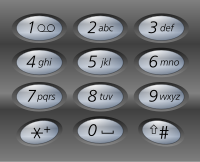
\includegraphics[width=.9\linewidth]{./pic/phoneNumber.png}
\caption{Letter Combinationas of Phone Number}
\end{figure}
\lstset{language=java,label= ,caption= ,numbers=none}
\begin{lstlisting}
Input:Digit string "23"
Output: ["ad", "ae", "af", "bd", "be", "bf", "cd", "ce", "cf"].
\end{lstlisting}
Note:

Although the above answer is in lexicographical order, your answer could be in any order you want.
\subsection{Restore IP Addresses}
\label{sec-6-4-2}
Given a string containing only digits, restore it by returning all possible valid IP address combinations.

For example:
\lstset{language=java,label= ,caption= ,numbers=none}
\begin{lstlisting}
Given "25525511135",
return ["255.255.11.135", "255.255.111.35"]. (Order does not matter)
\end{lstlisting}
\subsection{Generate Parentheses}
\label{sec-6-4-3}
Given n pairs of parentheses, write a function to generate all combinations of well-formed parentheses.

For example, given n = 3, a solution set is:
\lstset{language=java,label= ,caption= ,numbers=none}
\begin{lstlisting}
"((()))", "(()())", "(())()", "()(())", "()()()"
\end{lstlisting}
\subsection{Gray Code}
\label{sec-6-4-4}
The gray code is a binary numeral system where two successive values differ in only one bit.

Given a non-negative integer n representing the total number of bits in the code, print the sequence of gray code. A gray code sequence must begin with 0.

For example, given n = 2, return [0,1,3,2]. Its gray code sequence is:
\lstset{language=java,label= ,caption= ,numbers=none}
\begin{lstlisting}
00 - 0
01 - 1
11 - 3
10 - 2
\end{lstlisting}
Note:
\begin{itemize}
\item For a given n, a gray code sequence is not uniquely defined.
\item For example, [0,2,3,1] is also a valid gray code sequence according to the above definition.
\item For now, the judge is able to judge based on one instance of gray code sequence. Sorry about that.
\end{itemize}
\subsection{Word Search}
\label{sec-6-4-5}
Given a 2D board and a word, find if the word exists in the grid.

The word can be constructed from letters of sequentially adjacent cell, where "adjacent" cells are those horizontally or vertically neighboring. The same letter cell may not be used more than once.

For example,
\lstset{language=java,label= ,caption= ,numbers=none}
\begin{lstlisting}
Given board =
[
  ["ABCE"],
  ["SFCS"],
  ["ADEE"]
]
word = "ABCCED", -> returns true,
word = "SEE", -> returns true,
word = "ABCB", -> returns false.
\end{lstlisting}
\subsection{Palindrome Partitioning}
\label{sec-6-4-6}
Given a string s, partition s such that every substring of the partition is a palindrome.

Return all possible palindrome partitioning of s.

For example, 
\lstset{language=java,label= ,caption= ,numbers=none}
\begin{lstlisting}
given s = "aab",
Return
  [
    ["aa","b"],
    ["a","a","b"]
  ]
\end{lstlisting}
\subsection{N-Queens}
\label{sec-6-4-7}
The n-queens puzzle is the problem of placing n queens on an n×n chessboard such that no two queens attack each other.
\begin{figure}[htb]
\centering
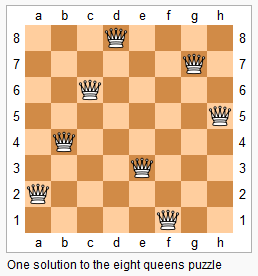
\includegraphics[width=.9\linewidth]{./pic/8-queens.png}
\caption{N-Queens}
\end{figure}

Given an integer n, return all distinct solutions to the n-queens puzzle.

Each solution contains a distinct board configuration of the n-queens' placement, where 'Q' and '.' both indicate a queen and an empty space respectively.

For example,

There exist two distinct solutions to the 4-queens puzzle:
\lstset{language=java,label= ,caption= ,numbers=none}
\begin{lstlisting}
[
 [".Q..",  // Solution 1
  "...Q",
  "Q...",
  "..Q."],

 ["..Q.",  // Solution 2
  "Q...",
  "...Q",
  ".Q.."]
]
\end{lstlisting}
\subsection{N-Queens II}
\label{sec-6-4-8}
Follow up for N-Queens problem.

Now, instead outputting board configurations, return the total number of distinct solutions.
\subsection{Sudoku Solver}
\label{sec-6-4-9}
Write a program to solve a Sudoku puzzle by filling the empty cells.

Empty cells are indicated by the character '.'.

You may assume that there will be only one unique solution.

\begin{figure}[htb]
\centering
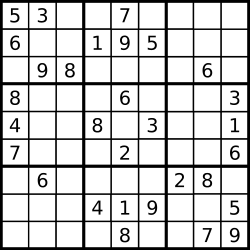
\includegraphics[width=.9\linewidth]{./pic/solveSudoku1.png}
\caption{Sudoku Solver 1}
\end{figure}
A sudoku puzzle\ldots{}

\begin{figure}[htb]
\centering
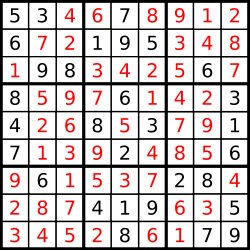
\includegraphics[width=.9\linewidth]{./pic/solveSudoku2.png}
\caption{Sudoku Solver 2}
\end{figure}
\ldots{}and its solution numbers marked in red.

\textbf{Tags:} Backtracking, Hash Table

\subsection{Regular Expression Matching}
\label{sec-6-4-10}
Implement regular expression matching with support for '.' and '*'.
\begin{itemize}
\item '.' Matches any single character.
\item '*' Matches zero or more of the preceding element.
\end{itemize}

The matching should cover the entire input string (not partial).

The function prototype should be:

bool isMatch(const char *s, const char *p)

Some examples:
\lstset{language=java,label= ,caption= ,numbers=none}
\begin{lstlisting}
isMatch("aa","a") → false
isMatch("aa","aa") → true
isMatch("aaa","aa") → false
isMatch("aa", "a*") → true
isMatch("aa", ".*") → true
isMatch("ab", ".*") → true
isMatch("aab", "c*a*b") → true
\end{lstlisting}
\textbf{Tags:} Dynamic Programming, Backtracking, String
\subsection{Wild Card Matching}
\label{sec-6-4-11}
Implement wildcard pattern matching with support for '?' and '*'.
\begin{itemize}
\item '?' Matches any single character.
\item '*' Matches any sequence of characters (including the empty sequence).
\end{itemize}

The matching should cover the entire input string (not partial).

The function prototype should be:

bool isMatch(const char *s, const char *p)

Some examples:
\lstset{language=java,label= ,caption= ,numbers=none}
\begin{lstlisting}
isMatch("aa","a") → false
isMatch("aa","aa") → true
isMatch("aaa","aa") → false
isMatch("aa", "*") → true
isMatch("aa", "a*") → true
isMatch("ab", "?*") → true
isMatch("aab", "c*a*b") → false
\end{lstlisting}
\textbf{Tags:} Dynamic Programming, Backtracking, Greedy, String
\subsection{Word Break II}
\label{sec-6-4-12}
Given a string s and a dictionary of words dict, add spaces in s to construct a sentence where each word is a valid dictionary word.

Return all such possible sentences.

For example, given
\lstset{language=java,label= ,caption= ,numbers=none}
\begin{lstlisting}
s = "catsanddog",
dict = ["cat", "cats", "and", "sand", "dog"].

A solution is ["cats and dog", "cat sand dog"].
\end{lstlisting}
\textbf{Tags:} Dynamic Programming Backtracking

\subsection{Word Ladder II}
\label{sec-6-4-13}
Given two words (start and end), and a dictionary, find all shortest transformation sequence(s) from start to end, such that:
\begin{itemize}
\item Only one letter can be changed at a time
\item Each intermediate word must exist in the dictionary
\end{itemize}
For example,
\lstset{language=java,label= ,caption= ,numbers=none}
\begin{lstlisting}
Given:
start = "hit"
end = "cog"
dict = ["hot","dot","dog","lot","log"]
Return
  [
    ["hit","hot","dot","dog","cog"],
    ["hit","hot","lot","log","cog"]
  ]
\end{lstlisting}
Note:
\begin{itemize}
\item All words have the same length.
\item All words contain only lowercase alphabetic characters.
\end{itemize}
\textbf{Tags:} Array, Backtracking, Breadth-first Search, String

\chapter{Bit Manipulation}
\label{sec-7}
\subsection{Subsets: Bit Manipulation}
\label{sec-7-0-1}
Given a set of distinct integers, S, return all possible subsets.

Note:
\begin{itemize}
\item Elements in a subset must be in non-descending order.
\item The solution set must not contain duplicate subsets.
\end{itemize}
For example,
If S = [1,2,3], a solution is:
\lstset{language=java,label= ,caption= ,numbers=none}
\begin{lstlisting}
[
  [3],
  [1],
  [2],
  [1,2,3],
  [1,3],
  [2,3],
  [1,2],
  []
]
\end{lstlisting}
\textbf{Tags:} Array Backtracking, Bit Manipulation
\subsection{Single Number}
\label{sec-7-0-2}
\subsection{Single Number II}
\label{sec-7-0-3}
\subsection{Majority Element}
\label{sec-7-0-4}
\chapter{排序}
\label{sec-8}

\chapter{查找: Binary Search}
\label{sec-9}
\section{Easier Maybe?}
\label{sec-9-1}
\subsection{Search Insert Position}
\label{sec-9-1-1}
\subsection{Find Minimum in Rotated Sorted Array}
\label{sec-9-1-2}
\subsection{Find Minimum in Rotated Sorted Array II - with Duplicates}
\label{sec-9-1-3}
\subsection{}
\label{sec-9-1-4}
\chapter{暴力枚举法}
\label{sec-10}

\subsection{}
\label{sec-10-0-1}
\chapter{广度优先搜索: Breadth First Search}
\label{sec-11}
\subsection{Word Ladder}
\label{sec-11-0-1}
Given two words (start and end), and a dictionary, find the length of shortest transformation sequence from start to end, such that:
\begin{itemize}
\item Only one letter can be changed at a time
\item Each intermediate word must exist in the dictionary
\end{itemize}
For example,

Given:
\lstset{language=java,label= ,caption= ,numbers=none}
\begin{lstlisting}
start = "hit"
end = "cog"
dict = ["hot","dot","dog","lot","log"]
As one shortest transformation is "hit" -> "hot" -> "dot" -> "dog" -> "cog",
return its length 5.
\end{lstlisting}
Note:
\begin{itemize}
\item Return 0 if there is no such transformation sequence.
\item All words have the same length.
\item All words contain only lowercase alphabetic characters.
\end{itemize}
\subsection{}
\label{sec-11-0-2}
\chapter{深度优先搜索: Depth First Search}
\label{sec-12}

\chapter{分治法: Divide and Conqure}
\label{sec-13}
\subsection{Maximum Subarray}
\label{sec-13-0-1}
\subsection{Merge K sorted List}
\label{sec-13-0-2}
\subsection{Median of Two Sorted Array}
\label{sec-13-0-3}
\subsection{Majority Element}
\label{sec-13-0-4}
\subsection{}
\label{sec-13-0-5}
\subsection{}
\label{sec-13-0-6}
\subsection{}
\label{sec-13-0-7}
\chapter{贫心法: Greedy Search}
\label{sec-14}
\subsection{Gas Station}
\label{sec-14-0-1}
\subsection{Best Time to Buy and Sell Stock II}
\label{sec-14-0-2}
\subsection{Jump Game}
\label{sec-14-0-3}
\subsection{Jump Game II}
\label{sec-14-0-4}
\subsection{Candy}
\label{sec-14-0-5}
\subsection{Wildcard Matching}
\label{sec-14-0-6}
\subsection{}
\label{sec-14-0-7}

\chapter{动态归划:Dynamic Programming}
\label{sec-15}
\subsection{Climbing Stairs}
\label{sec-15-0-1}
\subsection{Unique Path}
\label{sec-15-0-2}
\subsection{Unique Path II}
\label{sec-15-0-3}
\subsection{Maximum Sum Subarray}
\label{sec-15-0-4}
\subsection{Maximum Product Subarray}
\label{sec-15-0-5}
\subsection{Coins in a Line}
\label{sec-15-0-6}
\subsection{Word Break}
\label{sec-15-0-7}
Given a string s and a dictionary of words dict, determine if s can be segmented into a space-separated sequence of one or more dictionary words.

For example, given
\lstset{language=java,label= ,caption= ,numbers=none}
\begin{lstlisting}
s = "leetcode",
dict = ["leet", "code"].
Return true because "leetcode" can be segmented as "leet code".
\end{lstlisting}
\subsection{Palindrome Partitioning II}
\label{sec-15-0-8}
Given a string s, partition s such that every substring of the partition is a palindrome.

Return the minimum cuts needed for a palindrome partitioning of s.

For example, 
\lstset{language=java,label= ,caption= ,numbers=none}
\begin{lstlisting}
given s = "aab",
Return 1 since the palindrome partitioning ["aa","b"] could be produced using 1 cut.
\end{lstlisting}

\chapter{Two Pointers and Sliding Window}
\label{sec-16}
\subsection{}
\label{sec-16-0-1}

\chapter{图: Graphics}
\label{sec-17}
\section{Clone Graph}
\label{sec-17-1}
Clone an undirected graph. Each node in the graph contains a label and a list of its neighbors.

OJ's undirected graph serialization:

Nodes are labeled uniquely.

We use \# as a separator for each node, and , as a separator for node label and each neighbor of the node.

As an example, consider the serialized graph \{0,1,2\#1,2\#2,2\}.

The graph has a total of three nodes, and therefore contains three parts as separated by \#.

\begin{enumerate}
\item First node is labeled as 0. Connect node 0 to both nodes 1 and 2.
\item Second node is labeled as 1. Connect node 1 to node 2.
\item Third node is labeled as 2. Connect node 2 to node 2 (itself), thus forming a self-cycle.
\end{enumerate}

Visually, the graph looks like the following:
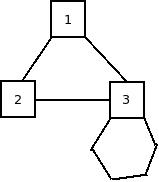
\includegraphics[width=.9\linewidth]{./pic/clonegraph.jpg}

\subsection{分析: 广度优先遍历或深度优先遍历都可以}
\label{sec-17-1-1}
\subsection{DFS: 时间复杂度O(n), 空间复杂度O(n)}
\label{sec-17-1-2}
\lstset{language=java,label= ,caption= ,numbers=none}
\begin{lstlisting}
/**
 * Definition for undirected graph.
 * class UndirectedGraphNode {
 *     int label;
 *     List<UndirectedGraphNode> neighbors;
 *     UndirectedGraphNode(int x) { label = x; neighbors = new ArrayList<UndirectedGraphNode>(); }
 * };
 */
public UndirectedGraphNode cloneGraph(UndirectedGraphNode node) {
    if (node == null) return null;
    UndirectedGraphNode res = new UndirectedGraphNode(node.label);  // result head
    if (node.neighbors == null || node.neighbors.size() == 0) return res;

    Map<UndirectedGraphNode, UndirectedGraphNode> map = new HashMap<UndirectedGraphNode, UndirectedGraphNode>();
    Queue<UndirectedGraphNode> q = new LinkedList<UndirectedGraphNode>();
    q.add(node);                      // added first node, need add its all Neighbors as well
    map.put(node, res);

    List<UndirectedGraphNode> curNbr = new ArrayList<UndirectedGraphNode>();
    UndirectedGraphNode curr = null;
    while (!q.isEmpty()) {
        curr = q.poll();
        curNbr = curr.neighbors;                   // ori
        for (UndirectedGraphNode aNbr : curNbr) {  // for build connection among copies
            if (!map.containsKey(aNbr)) {
                UndirectedGraphNode acpNbr = new UndirectedGraphNode(aNbr.label);
                map.put(aNbr, acpNbr);
                map.get(curr).neighbors.add(acpNbr);
                q.add(aNbr);
            } else
                map.get(curr).neighbors.add(map.get(aNbr));                        
        }
    }
    return res;
}
\end{lstlisting}
\subsection{BFS:}
\label{sec-17-1-3}
\section{Word Ladder, Word Ladder II: Backtracing}
\label{sec-17-2}
\subsection{Word Ladder}
\label{sec-17-2-1}
Given two words (start and end), and a dictionary, find the length of shortest transformation sequence from start to end, such that:
\begin{enumerate}
\item Only one letter can be changed at a time
\item Each intermediate word must exist in the dictionary
\end{enumerate}

For example,

Given:
start = "hit", end = "cog"

dict = ["hot","dot","dog","lot","log"]

As one shortest transformation is "hit" -> "hot" -> "dot" -> "dog" -> "cog",

return its length 5.

Note:
\begin{itemize}
\item Return 0 if there is no such transformation sequence.
\item All words have the same length.
\item All words contain only lowercase alphabetic characters.
\end{itemize}

\subsection{Word Ladder II}
\label{sec-17-2-2}
Given two words (start and end), and a dictionary, find all shortest transformation sequence(s) from start to end, such that:
\begin{enumerate}
\item Only one letter can be changed at a time
\item Each intermediate word must exist in the dictionary
\end{enumerate}
For example,

Given:

start = "hit", end = "cog"

dict = ["hot","dot","dog","lot","log"]

Return
\lstset{language=java,label= ,caption= ,numbers=none}
\begin{lstlisting}
[
  ["hit","hot","dot","dog","cog"],
  ["hit","hot","lot","log","cog"]
]
\end{lstlisting}

Note:
\begin{itemize}
\item All words have the same length.
\item All words contain only lowercase alphabetic characters.
\end{itemize}

\section{Check whether the graph is bigraph}
\label{sec-17-3}
\section{Topological Sort}
\label{sec-17-4}
Topological sorting for Directed Acyclic Graph (DAG) is a linear
ordering of vertices such that for every directed edge uv, vertex u
comes before v in the ordering. Topological Sorting for a graph is not
possible if the graph is not a DAG.

For example, a topological sorting of the following graph is “5 4 2 3
1 0″. There can be more than one topological sorting for a graph. For
example, another topological sorting of the following graph is “4 5 2
3 1 0″. The first vertex in topological sorting is always a vertex
with in-degree as 0 (a vertex with no in-coming edges).
\begin{figure}[htb]
\centering
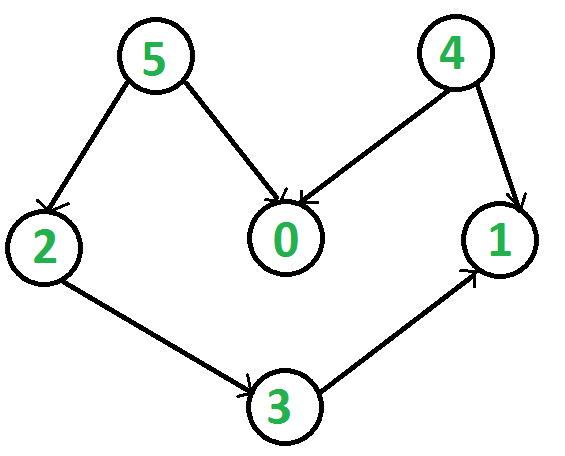
\includegraphics[width=.9\linewidth]{./pic/topologicalSorting.png}
\caption{Topological Sorting}
\end{figure}
\subsection{Topological Sorting vs Depth First Traversal (DFS):}
\label{sec-17-4-1}
In DFS, we print a vertex and then recursively call DFS for its adjacent vertices. In topological sorting, we need to print a vertex before its adjacent vertices. For example, in the given graph, the vertex ‘5’ should be printed before vertex ‘0’, but unlike DFS, the vertex ‘4’ should also be printed before vertex ‘0’. So Topological sorting is different from DFS. For example, a DFS of the above graph is “5 2 3 1 0 4″, but it is not a topological sorting.
\subsection{Algorithm to find Topological Sorting:}
\label{sec-17-4-2}
We recommend to first see implementation of DFS here. We can modify DFS to find Topological Sorting of a graph. In DFS, we start from a vertex, we first print it and then recursively call DFS for its adjacent vertices. In topological sorting, we use a temporary stack. We don’t print the vertex immediately, we first recursively call topological sorting for all its adjacent vertices, then push it to a stack. Finally, print contents of stack. Note that a vertex is pushed to stack only when all of its adjacent vertices (and their adjacent vertices and so on) are already in stack.


\chapter{Data Structure}
\label{sec-18}
\section{Min Stack}
\label{sec-18-1}
Design a stack that supports push, pop, top, and retrieving the minimum element in constant time.
\begin{itemize}
\item push(x) -- Push element x onto stack.
\item pop() -- Removes the element on top of the stack.
\item top() -- Get the top element.
\item getMin() -- Retrieve the minimum element in the stack.
\textbf{Tags:} Stack Data Structure
\end{itemize}
\lstset{language=java,label= ,caption= ,numbers=none}
\begin{lstlisting}
public static class MinStack {
    Stack<Integer> stack = new Stack<Integer>();
    Stack<Integer> minStack = new Stack<Integer>();
    public void push(int x) {
        stack.push(x);
        if (minStack.isEmpty() || x <= minStack.peek()) {
            minStack.push(x);
        }
    }

    public void pop() { // java boxing & unboxing, container, object specific methods
        if (stack.peek().intValue() == minStack.peek().intValue()) 
            minStack.pop();
        stack.pop();
    }

    public int top() {
        return stack.peek();
    }

    public int getMin() {
        if (!minStack.isEmpty()) return minStack.peek();
        else return -1;
    }
}
\end{lstlisting}
\section{LRU Cache}
\label{sec-18-2}
Design and implement a data structure for Least Recently Used (LRU) cache. It should support the following operations: get and set.
\begin{itemize}
\item get(key) - Get the value (will always be positive) of the key if the key exists in the cache, otherwise return -1.
\item set(key, value) - Set or insert the value if the key is not already
present. When the cache reached its capacity, it should invalidate
the least recently used item before inserting a new item.
\end{itemize}
\lstset{language=java,label= ,caption= ,numbers=none}
\begin{lstlisting}
public static class LRUCache {
    public class Node {
        int key;
        int value;
        Node prev;
        Node next;
        public Node(int x, int y){
            key = x;
            value = y;
        }
    }

    private HashMap<Integer, Node> hash;
    private int cap;
    private int number;
    Node head;
    Node tail;
    public LRUCache(int capacity) {
        cap = capacity;
        number = 0;
        head = new Node(-1, -1);
        head.prev = null;
        head.next = null;
        tail = head;
        hash = new HashMap<Integer, Node>(capacity); // so I can restrict a size !!
    }

    public int get(int key) {
        Node res = hash.get(new Integer(key)); // don't understand here
        if (res != null) {
            refresh(res);   // update usage frequence
            return res.value;
        } else return -1;
        /*
          if (hash.containsKey(key)) {
          //Node res = hash.get(new Integer(key)); // don't understand here
          Node res = hash.get(key);
          refresh(res);   // update usage frequence
          return res.value;
          } else {
          return -1;
          }
        */
    }

    // so still, must maintain a doubly-linked list to order usage frequency
    public  void refresh(Node tmp) {
        if (tmp == head.next) return; // it's head already

        Node temp = head.next;  // head node in the hash
        Node prevNode = tmp.prev;
        Node nextNode = tmp.next;
        // set to be most recently used~~ move the tmp node to be head.next, connections
        head.next = tmp;  
        tmp.prev = head;
        tmp.next = temp;
        temp.prev = tmp;
        prevNode.next = nextNode;
        if (nextNode != null) 
            nextNode.prev = prevNode;
        else tail = prevNode;   // remember tail as well 
    }

    public void set(int key, int value) {
        Node res = hash.get(new Integer(key));
        if (res != null) {
            refresh(res);
            res.value = value;
        } else {
            //if (!hash.containsKey(key)) { // another way of detecting existing
            Node prevNode = new Node(key, value); 
            Node temp;
            if (number == cap) { // remove tail;
                temp = tail.prev;
                hash.remove(tail.key);      // remember to remove from hash too !!!
                if (temp != null) {
                    temp.next = null;
                }
                tail.prev = null;
                tail = temp;
                number--;
            }
            // add to tail first
            tail.next = prevNode;
            prevNode.prev = tail;
            tail = prevNode;
            refresh(prevNode);
            hash.put(key, prevNode); 
            number++;  // count node numbers
        }
    }
}
\end{lstlisting}
\section{Two Sum III - data Structure Design}
\label{sec-18-3}
Design and implement a TwoSum class. It should support the following operations: add and find.
\begin{itemize}
\item add - Add the number to an internal data structure.
\item find - Find if there exists any pair of numbers which sum is equal to the value.
\end{itemize}
For example,
\lstset{language=java,label= ,caption= ,numbers=none}
\begin{lstlisting}
add(1); add(3); add(5);
find(4) -> true
find(7) -> false
\end{lstlisting}
\textbf{Tags:} Hash Table, Data Structure

\chapter{细节实现题}
\label{sec-19}

\chapter{Math}
\label{sec-20}
\section{Easy}
\label{sec-20-1}
\subsection{Reverse Integer}
\label{sec-20-1-1}
\subsection{Plus One}
\label{sec-20-1-2}
\subsection{Palindrome Number}
\label{sec-20-1-3}
\subsection{Next Permutation: Math}
\label{sec-20-1-4}
Implement next permutation, which rearranges numbers into the lexicographically next greater permutation of numbers.

If such arrangement is not possible, it must rearrange it as the lowest possible order (ie, sorted in ascending order).

The replacement must be in-place, do not allocate extra memory.

Here are some examples. Inputs are in the left-hand column and its
corresponding outputs are in the right-hand column.
\lstset{language=java,label= ,caption= ,numbers=none}
\begin{lstlisting}
1,2,3 → 1,3,2
3,2,1 → 1,2,3
1,1,5 → 1,5,1
\end{lstlisting}

\subsection{}
\label{sec-20-1-5}
\section{}
\label{sec-20-2}
% Emacs 24.3.1 (Org mode 8.2.7c)
\end{document}